\section{Abstract}

The nucleotide frequencies in protein-coding sequences is the result of the equilibrium between mutation and selection.
As a consequence, protein-coding sequences subjected to mutational bias at the nucleotide level, and evolving under selection at the amino-acids, will lean toward lower mutational bias when observed at the protein level.
Unfortunately, parametric \gls{codon} models developed to estimate the rate of evolution on amino-acids use the observed mutational bias at the protein level and don't take into account this effect.
Thus, such parametric \gls{codon} models are inherently misspecified to untangle mutation and selection, and they don’t estimate the mutational process reliably.
We also show that even if the mutational process is misspecified, parametric \gls{codon} models are able to estimate reliably the rate of evolution acting on amino-acids.
But if one wants to also estimate the mutational process, one need to use model where the rate of evolution is a tensor (95 parameters) instead of a single parameter.


\section{Introduction}


\section{Results}

\subsection{Model of evolution}

We seek to simulate the evolution of protein-coding sequences along a specie tree.
Starting with one sequence at the root of the tree, the sequences evolves independently along the different branches of the tree, until they reach the leaves.
At the end of the simulation, we get one sequence for each leaf of the tree, meaning one sequence per specie.
Such evolutionary process is an idealized version of the reality, in the sens that the whole heterogeneity of sequences in the population is wiped away, with only one sequence representing the whole population.
To make such idealized process more realistic, one can use population-genetic framework.
In population-genetics, a change in the whole population sequence, called \gls{substitution}, is modeled as the product of a mutation and a fixation.
A mutation only appear in one specific individual of the population, and a fixation is the probability that this specific individual is eventually a parent of all the population later in time.
One interesting result of population genetic is that the \gls{substitution} rate is equal to the mutation rate if the mutations are selectively \gls{neutral}.
If a mutation is favored (disfavored) by selection, the \gls{substitution} rate is higher (lower) than the \gls{neutral} rate.\\
For a protein-coding \acrshort{DNA} sequence, a \gls{substitution} is modeled as the product of mutation at the nucleotide level, and selection of the amino-acid level.
On one hand, the mutation rate between nucleotides as assumed to be same for all sites of the sequences.
On the other hand, the selection for amino-acids is not assumed to be the same for all sites of the sequences.
For example, an exterior site (solvent accessible residue) might favor hydrophilic amino-acids, and an interior site of the protein might favor hydrophobic amino-acids.

\begin{figure}[H]
    \centering
    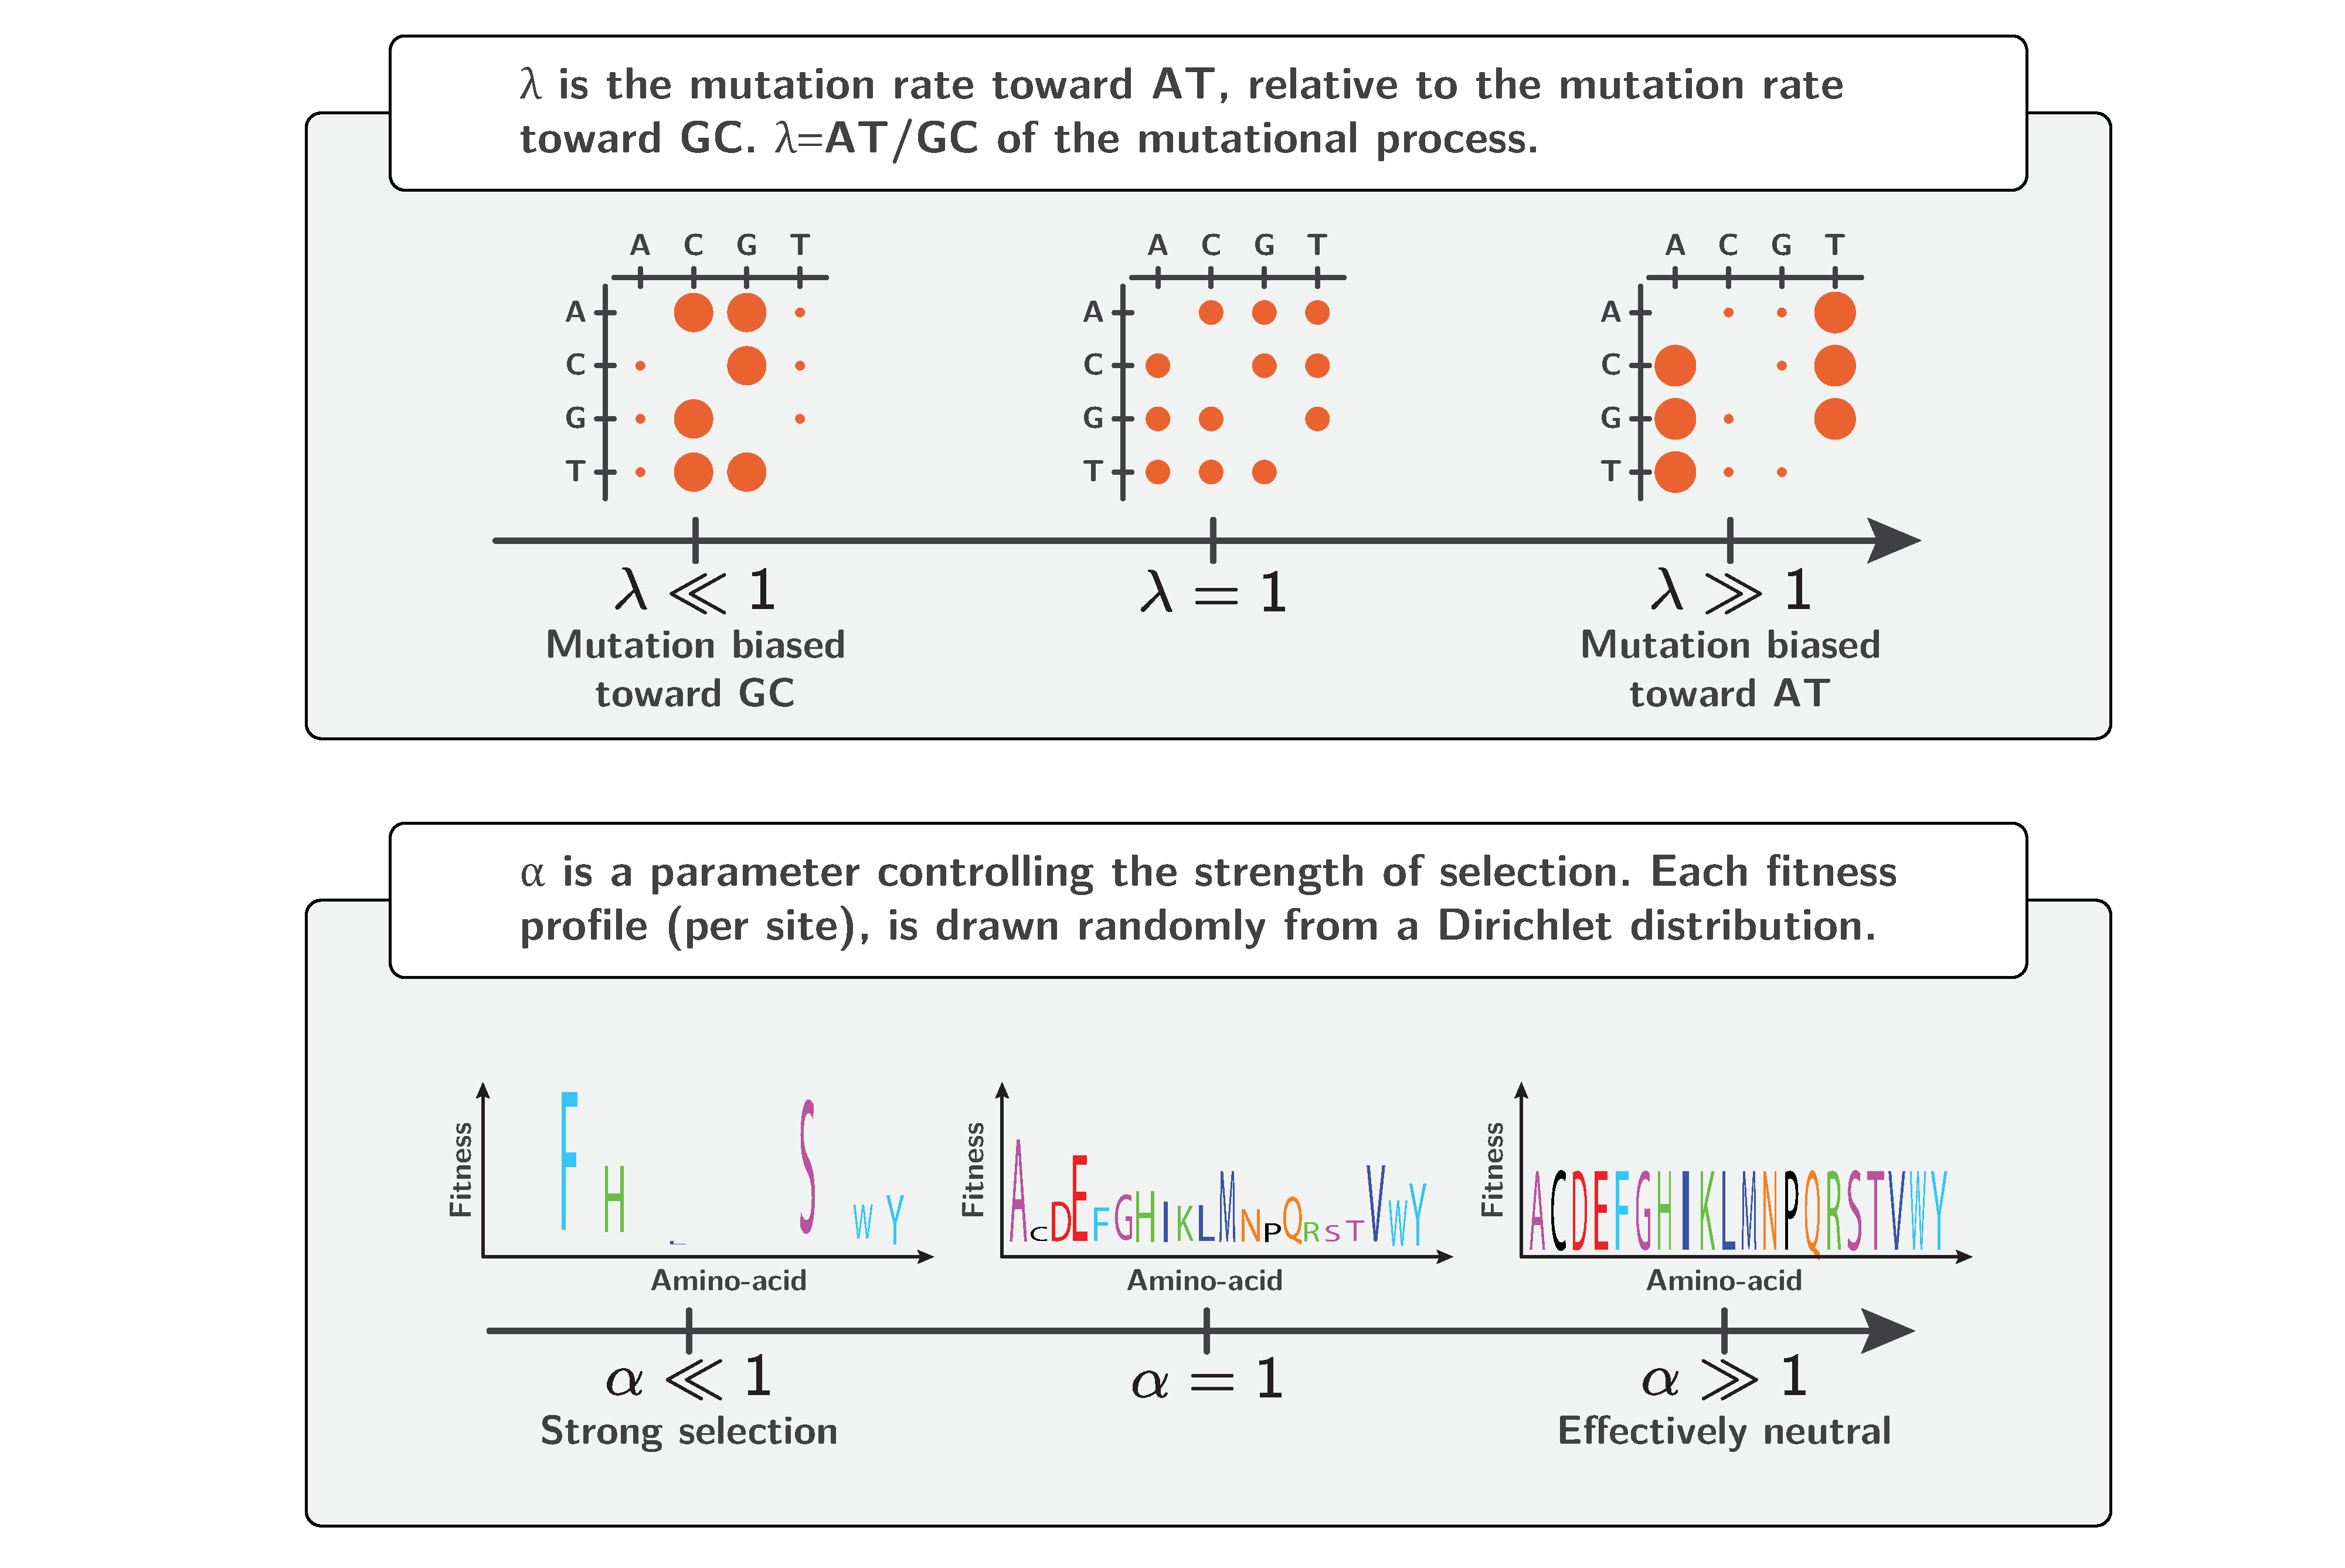
\includegraphics[width=\textwidth] {parameters}
    \caption[Parameters of the mutation-selection model]{
    Parameters of the mutation-selection model.
    One parameter for mutational bias, and one for strength of selection.}
\end{figure}

\subsection{Sumamry statistics}

\begin{figure}[H]
    \centering
    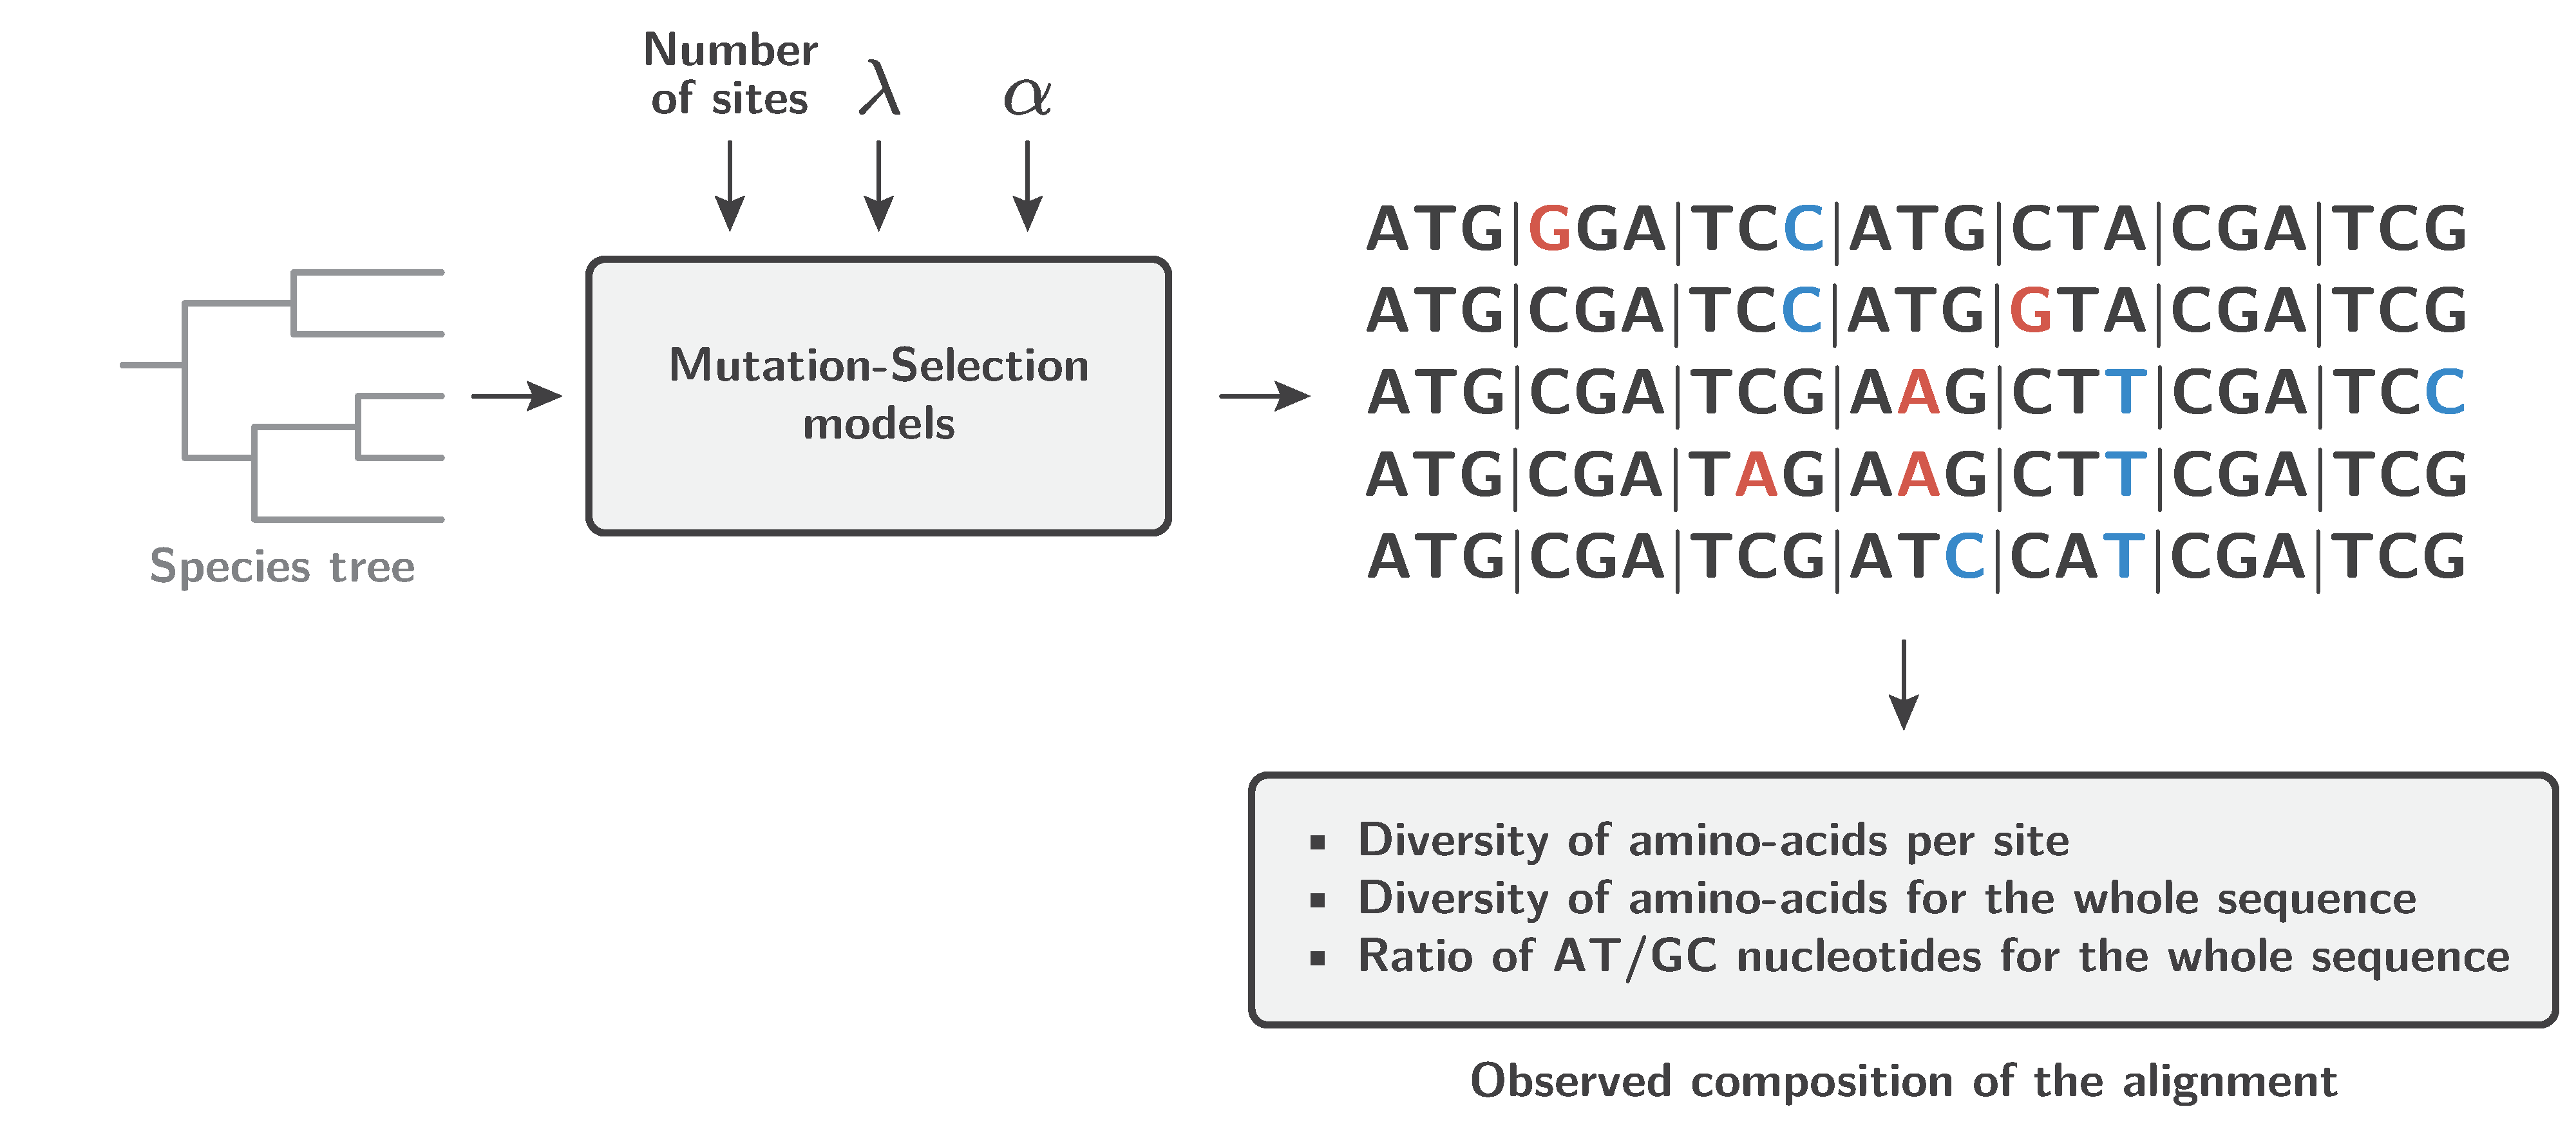
\includegraphics[width=\textwidth] {simulations-alignment}
    \caption[Simulations and analysis]{
    We can observe composition of the alignment as function of the mutation and selection parameters.}
\end{figure}

As noted in \ref{sec:mutBias}, the mutational process leads to $(\mutequi_A+\mutequi_T)/(\mutequi_C+\mutequi_G) = \lambda$.

\begin{figure}[H]
    \centering
    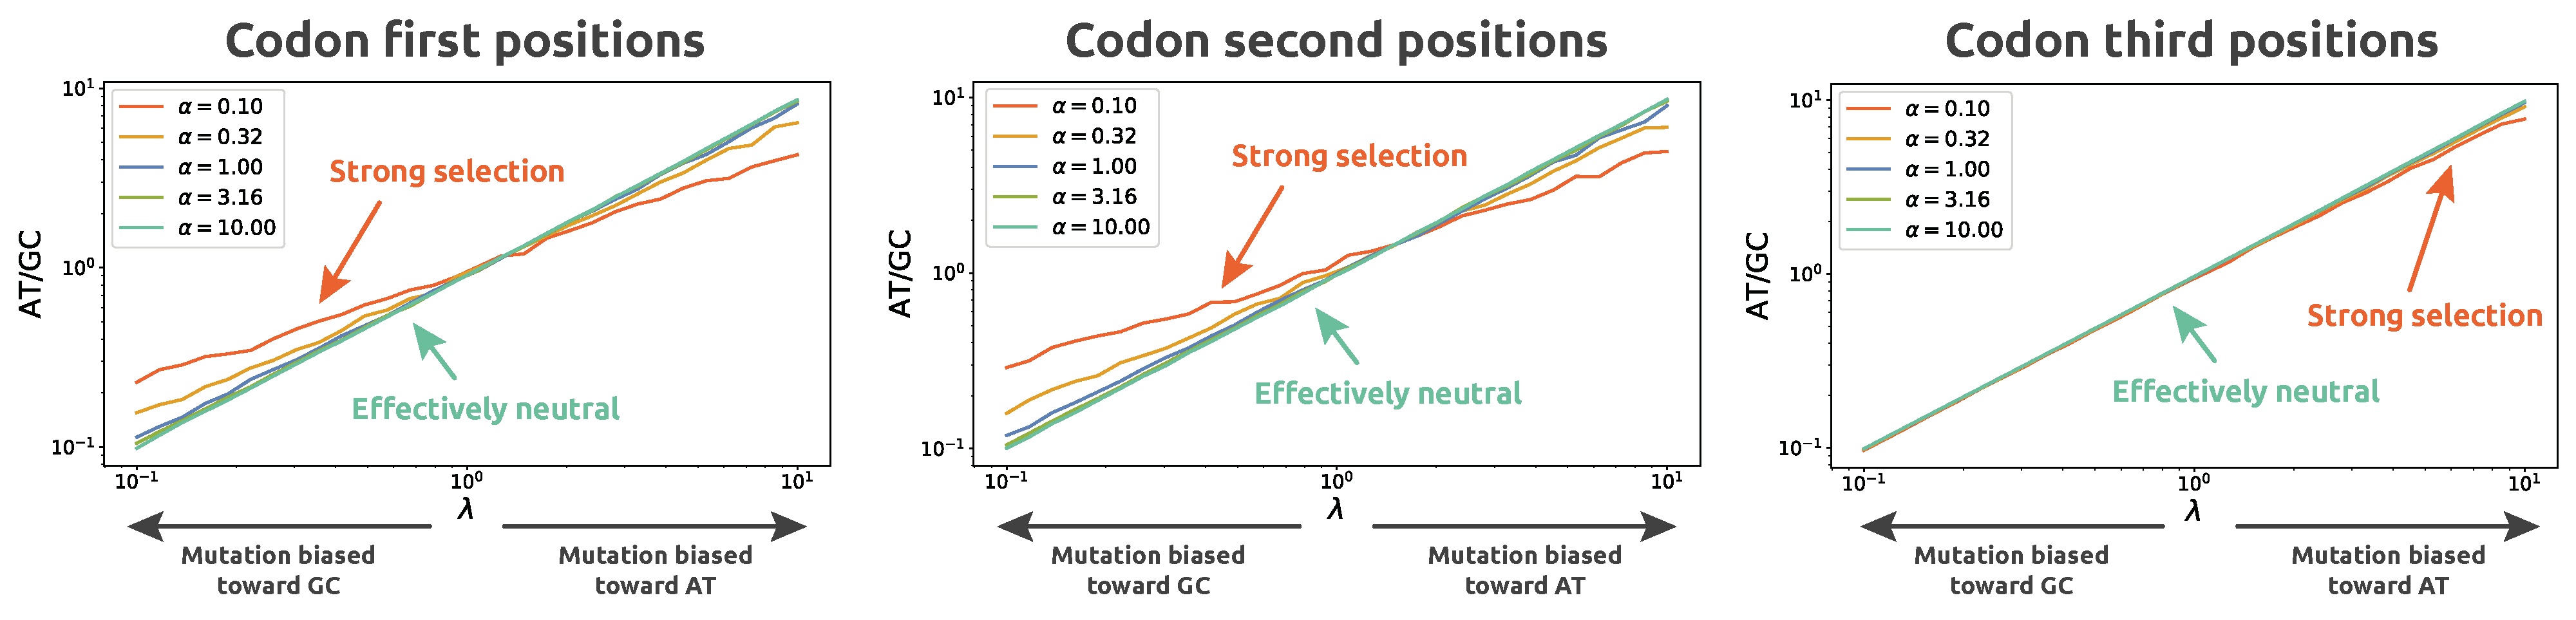
\includegraphics[width=\textwidth] {AT-GC-obs}
    \caption[AT/GC composition of the alignment]{
    AT/GC composition of the alignment.
    Observed AT/GC at the third \gls{codon} position matches the mutational bias.
    Selection is balancing the mutational bias.}
\end{figure}


The evolutionary variability of an amino acid site in a protein family is an important indicator of the selective constraints that the site experiences.
This variability is usually quantified through the sequence entropy \citep{Goldstein2017}.
Our analysis highlights how important it is to distinguish between amino acid frequencies averaged over a large class of sites and amino acid frequencies at individual sites.
In both cases, frequencies are Boltzmann distributed, and thus it is easy to mistake one for the other.
However, the properties of these two distributions are very different.
For example, all amino acids occur at comparable frequencies in the alignment, yet at any given site, only a small number of amino acids are actually permissible \citep{Ramsey2011}.

\begin{figure}[H]
    \centering
    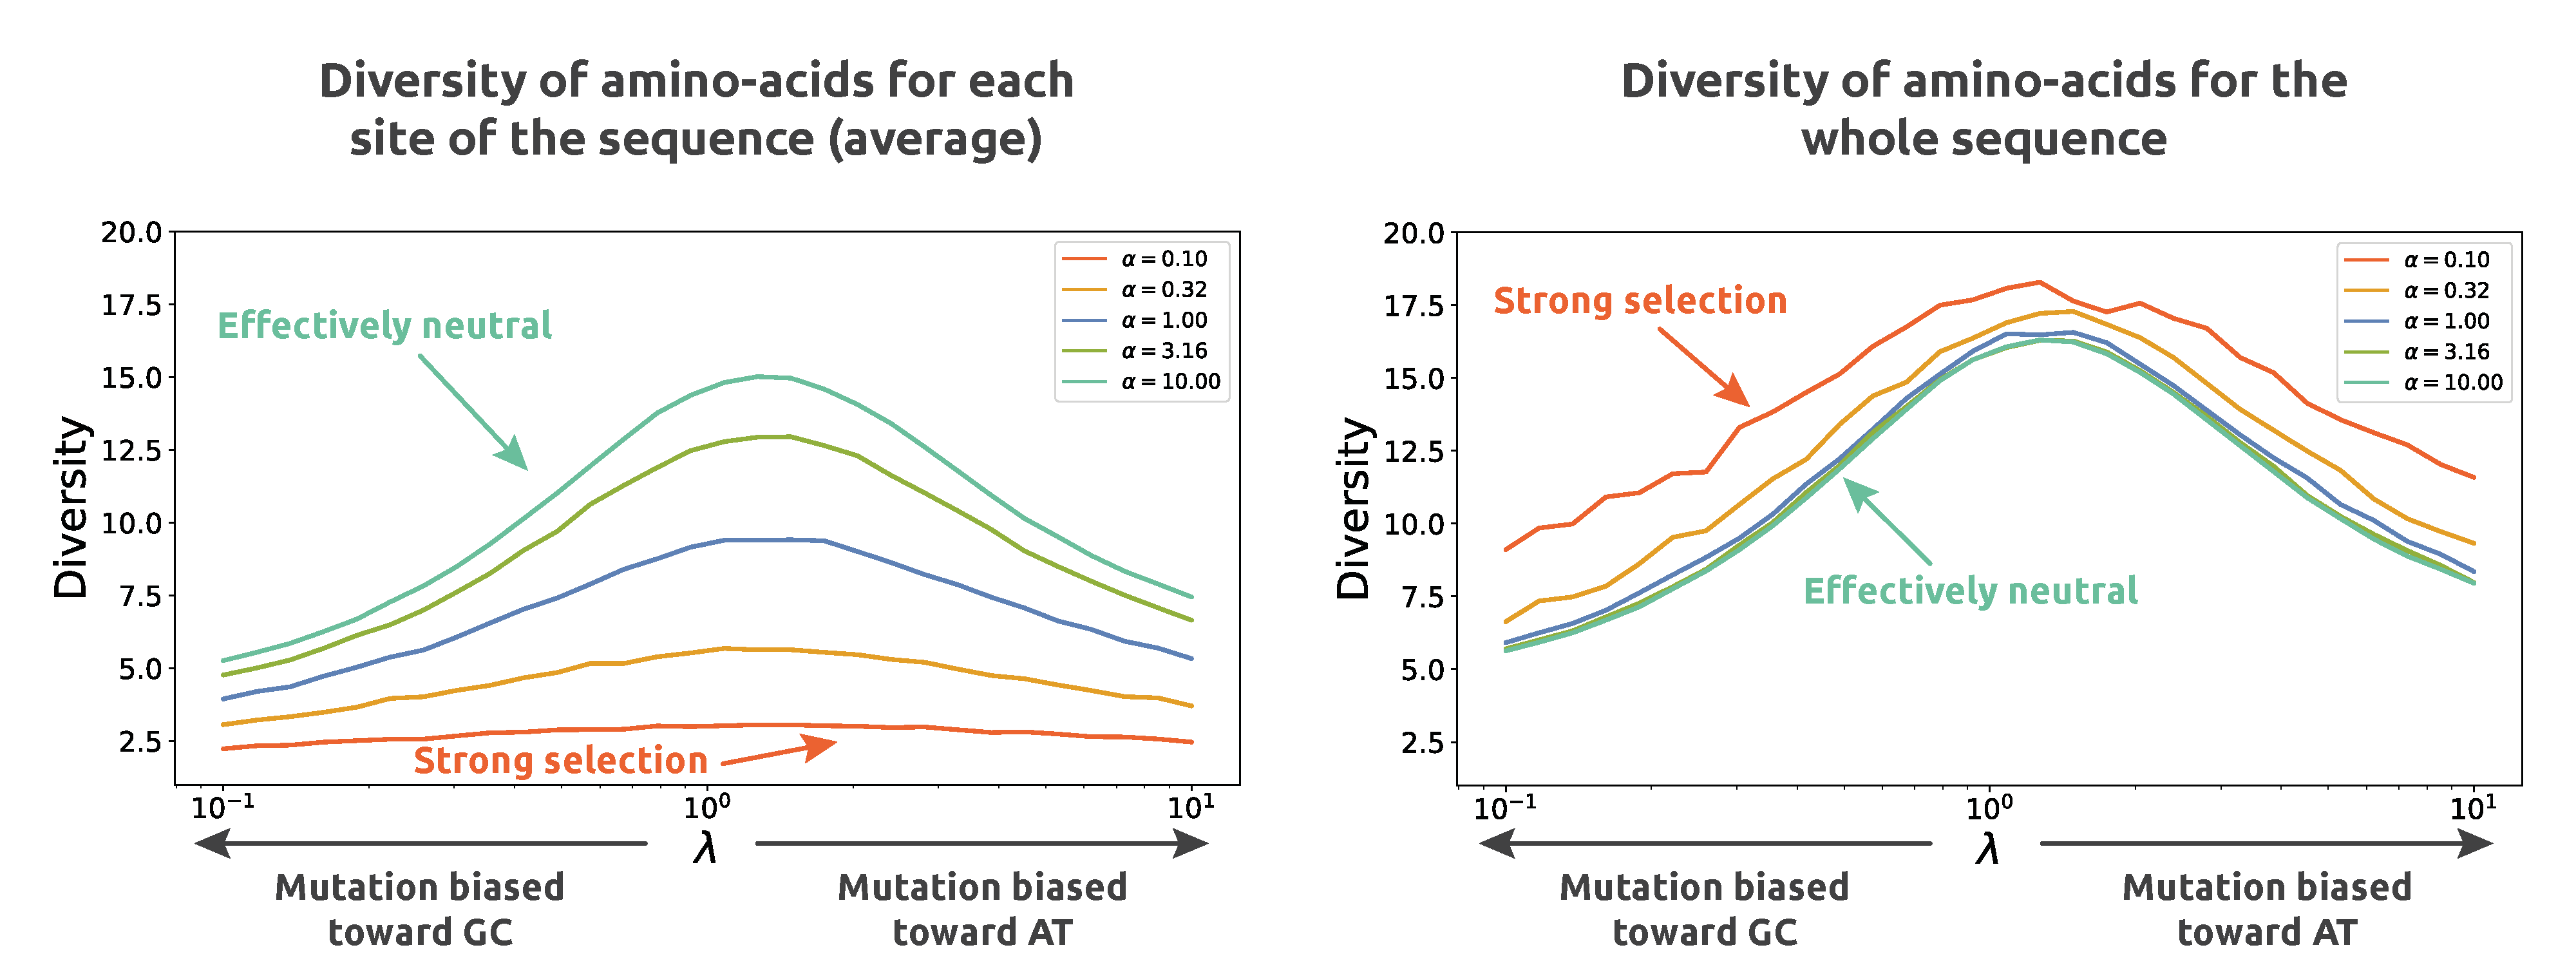
\includegraphics[width=\textwidth] {diversity-aa}
    \caption[Diversity of amino-acids]{
    Diversity of amino-acids, computed as the entropy of the amino-acid frequencies.
    Sequence-diversity is higher than site-diversity, because at any given site only a small number of amino acids are actually permissible.
    Diversity decreases with mutational bias.
    Site-diversity decreases with selection.
    Sequence-diversity increase with selection.}
\end{figure}

Evolutionary rate, which measures the rate at which mutations at individual sites arise and go to fixation, is governed by the amino acid distribution of individual sites, not the average distribution over a broad class of sites.
The \gls{substitution} rate (e.g., Grishin, Wolf \& Koonin, 2000).
These two measures of evolutionary variability are considered to be essentially equivalent \citep{Halpern1998}, though they are differently influenced by the mutational process \citep{Santos2018}.

\begin{figure}[H]
    \centering
    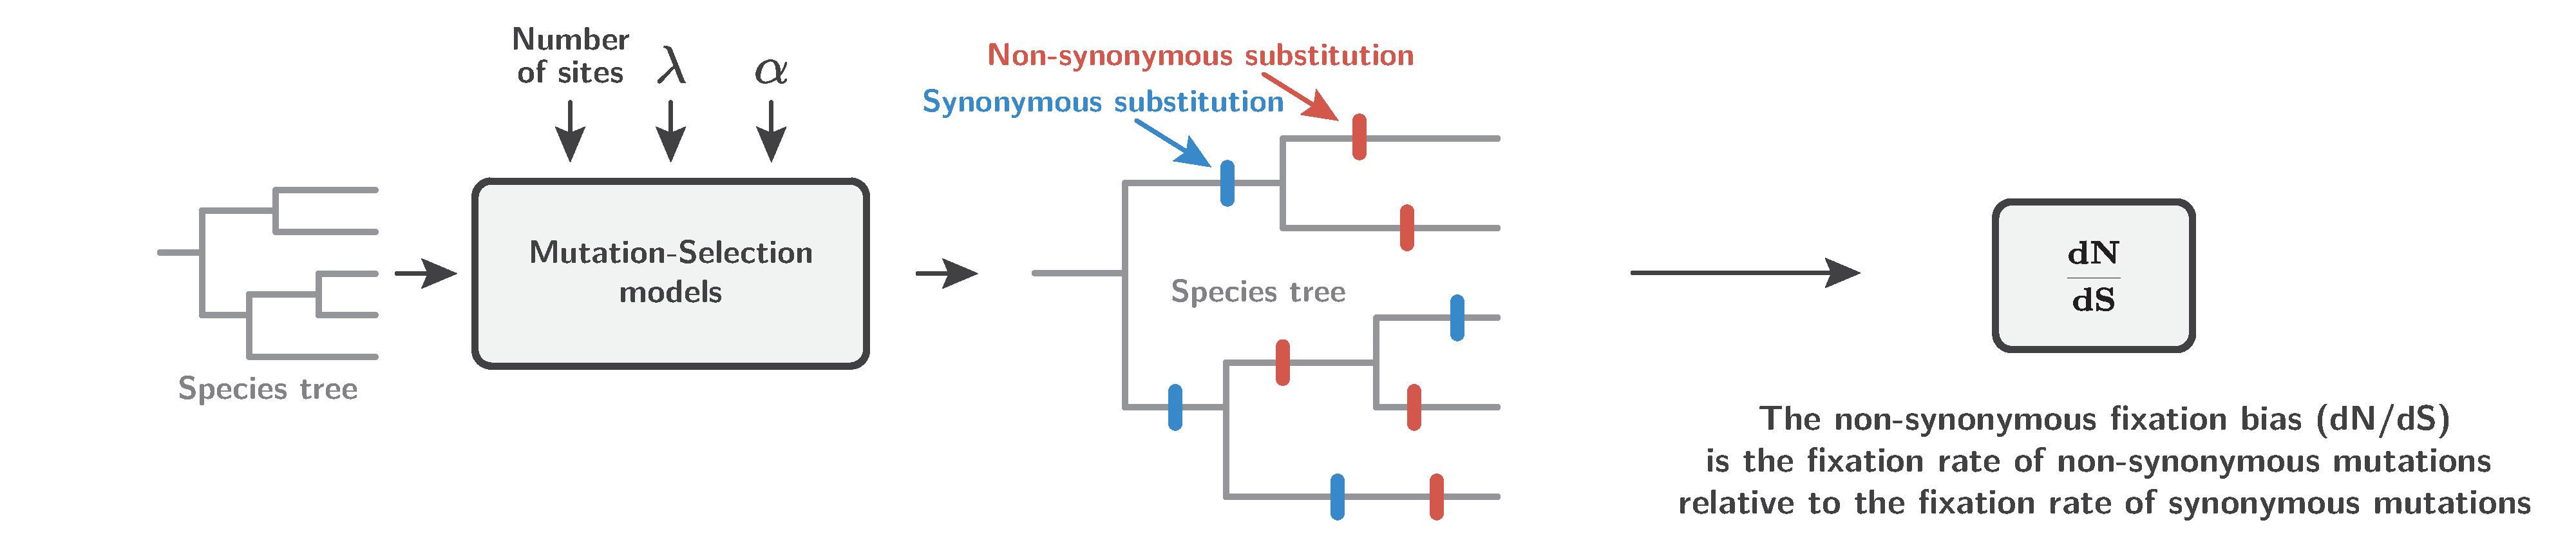
\includegraphics[width=\textwidth] {definitions-omega}

    \caption[Definition of $\omega$]{Definition of $\omega$.}
\end{figure}

\begin{figure}[H]
    \centering
    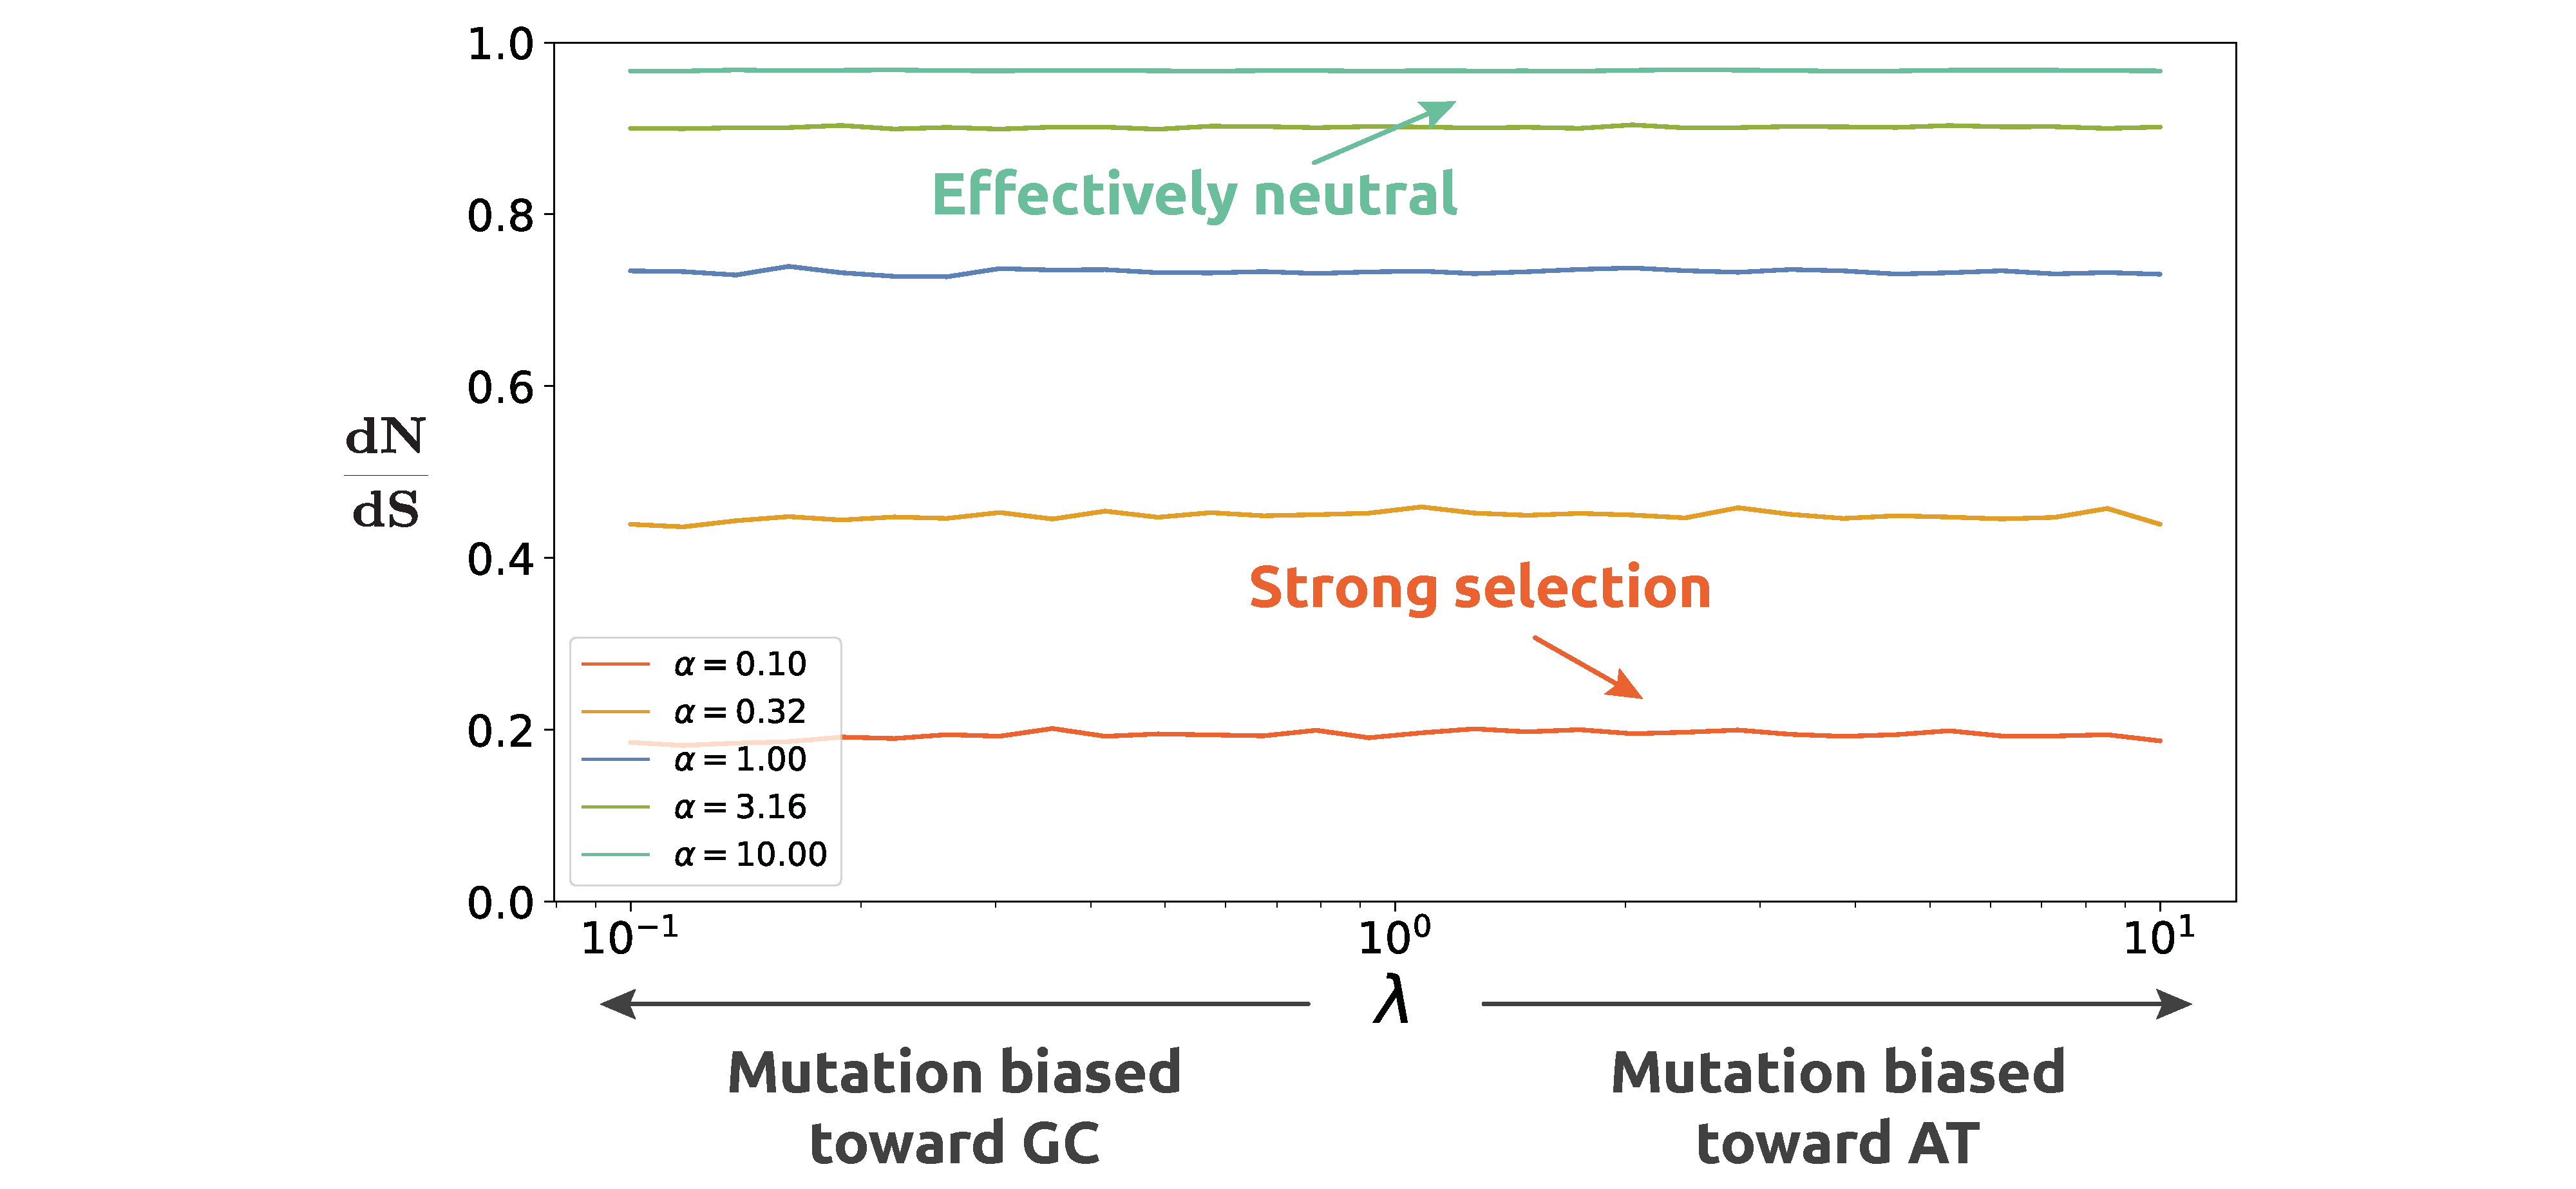
\includegraphics[width=\textwidth] {omega}

    \caption[$\omega$ as a function of the parameters]{
    $\omega$ as a function of the parameters.
    Non-synonymous fixation bias is always lower than.
    Non-synonymous fixation bias decrease with the strength of selection.
    Non-synonymous fixation bias is unaffected by mutational bias.}
\end{figure}

\begin{figure}[H]
    \centering
    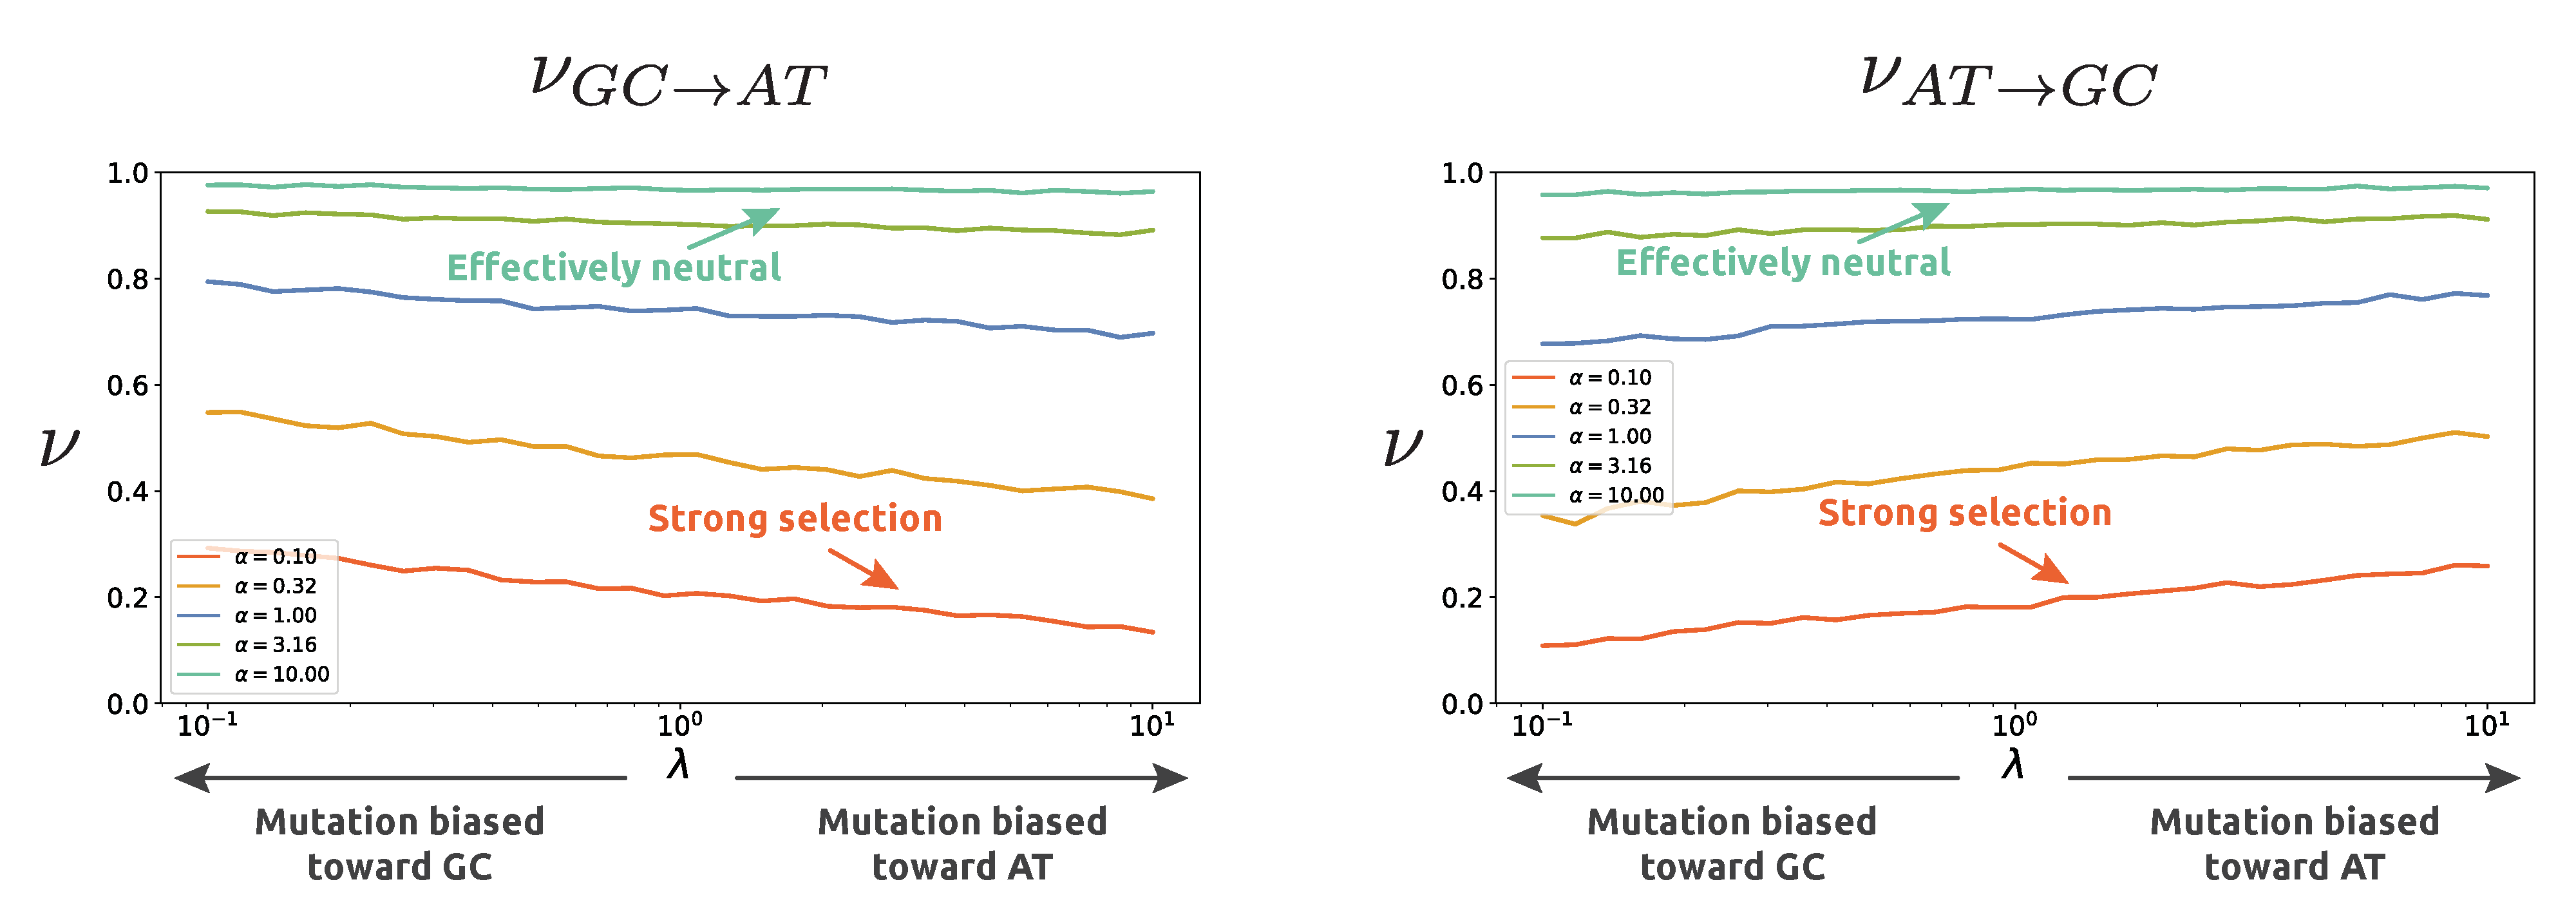
\includegraphics[width=\textwidth, page=1] {omega-WS-SW}

    \caption[Fixation bias of non-synonymous mutations]{
    Fixation bias of non-synonymous mutations.
    Mutation biased from GC to AT leads to a fixation bias in the opposite direction.
    More generally, mutation bias leads to balancing fixation bias.
    This is confounding factor with gBGC.}
\end{figure}

\subsection{Parametric inference with mean-field codon model}

\begin{figure}[H]
    \centering
    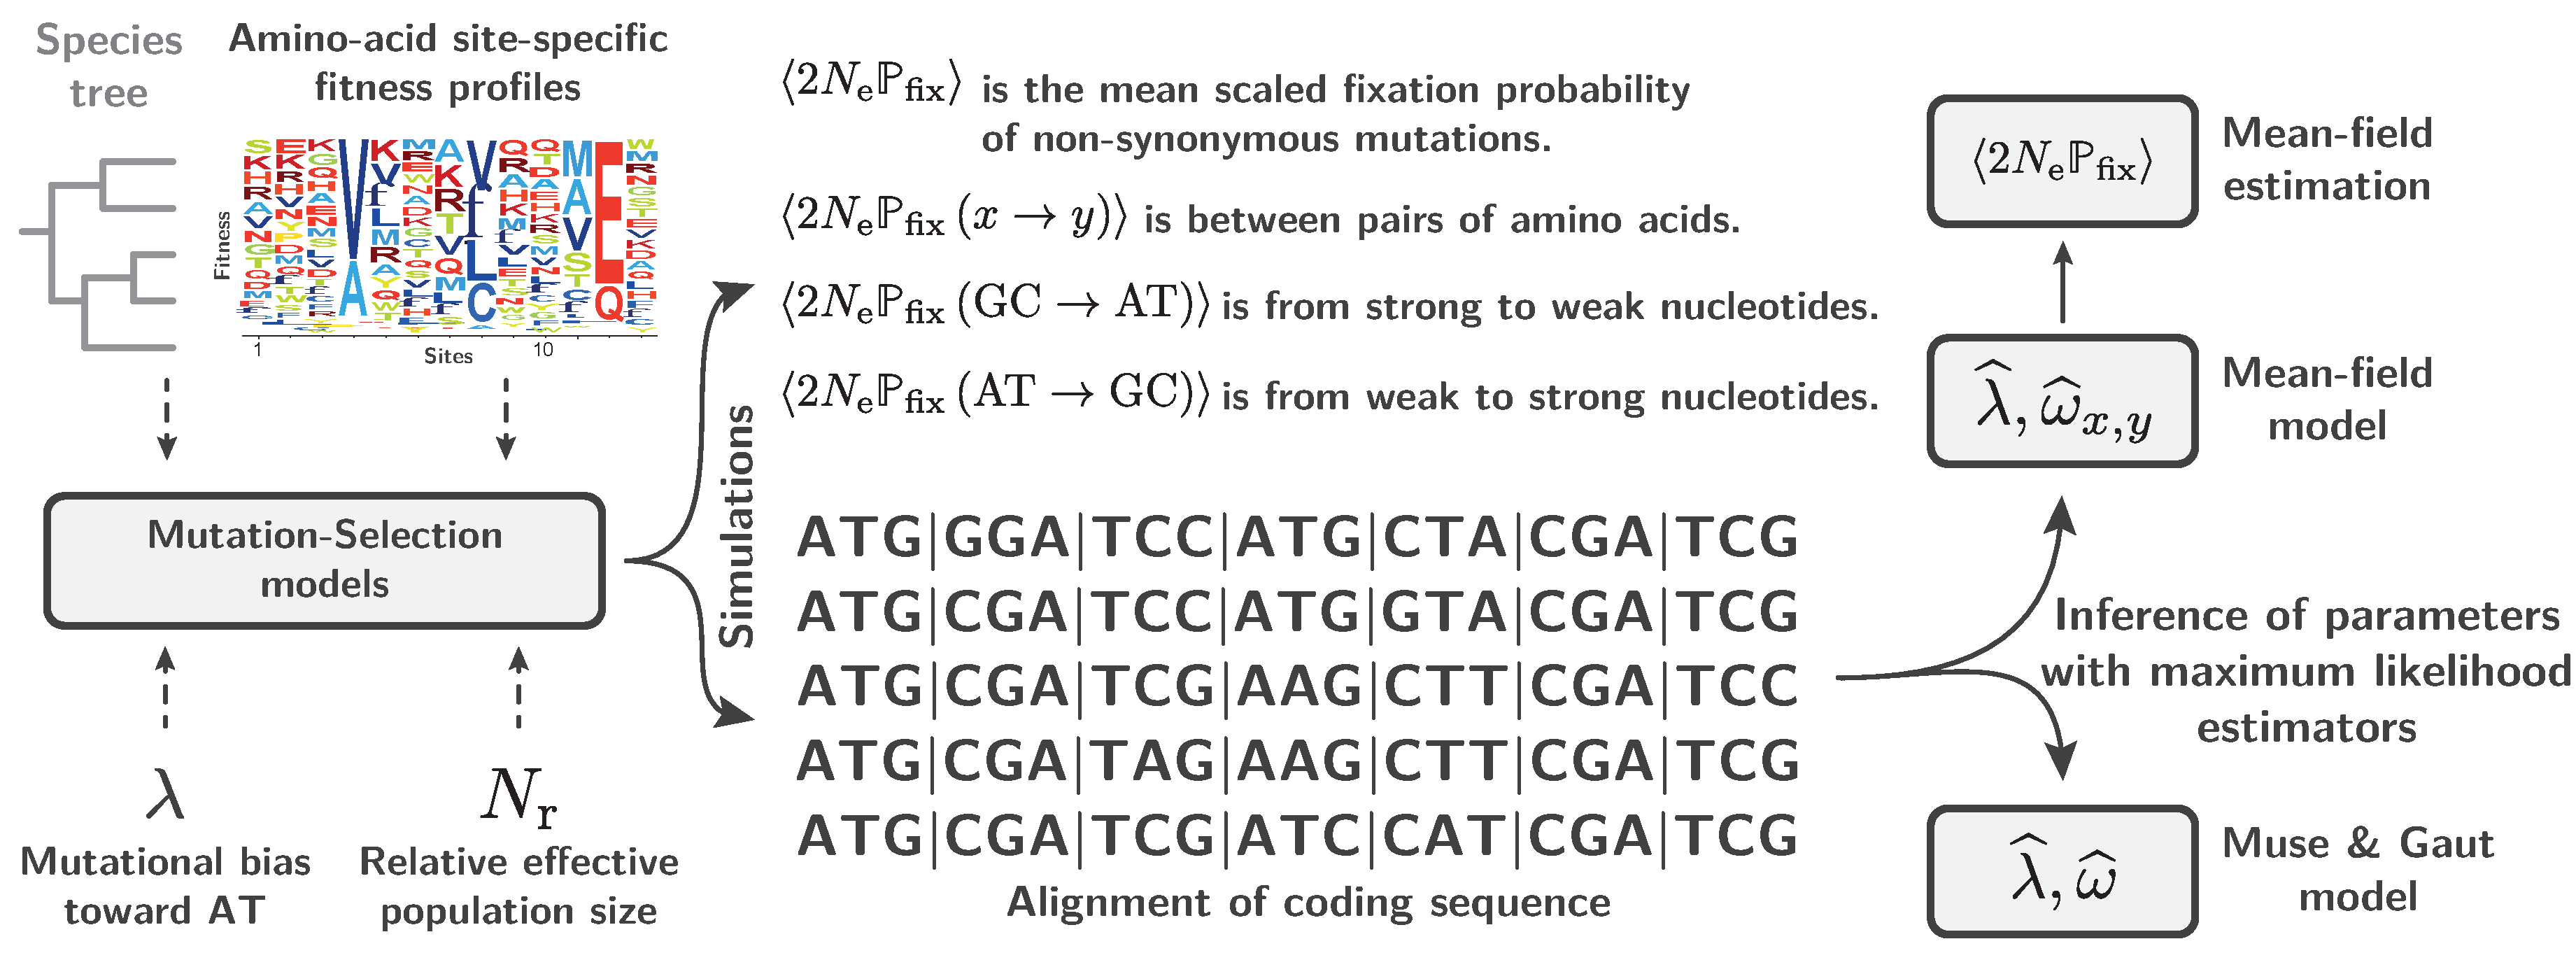
\includegraphics[width=\textwidth, page=1] {pipeline}
    \caption[Inferred value compared to known value]{
    Inferred value compared to known value.}
\end{figure}

The $61$-by-$61$ \gls{codon} \gls{substitution} matrix of \citet{Muse1994} is defined entirely by the mutation matrix ($\Mutmatrix$), $\omega$ and the genetic code:
\begin{equation}
    \begin{dcases}
        \submatrix_{\itoj} & = 0 \text{ if $\ci$ and $\cj$ are not one mutation away} \\
        \submatrix_{\itoj} & = \mutmatrix_{\nucitoj} \text{ if $\ci$ and $\cj$ are syonymous} \\
        \submatrix_{\itoj} & = \omega \mutmatrix_{\nucitoj} \text{ if $\ci$ and $\cj$ are non-syonymous} \\
        \submatrix_{\ci, \ci} & = - \sum_{\cj \neq \ci} \submatrix_{\itoj}
    \end{dcases}
    \label{eq:codon-muse-gaut}
\end{equation}

From the maximum \gls{likelihood} estimates of the $4 \times 4$ mutation matrix ($\widehat{\Mutmatrix}$), we can estimate of the mutational bias toward $\mathrm{AT}$ $\left({\widehat{\lambda}_{\text{MG}}} \right)$.
We can also estimate the fixation bias of non-synonymous mutations (${\widehat{\omega}_{\text{MG}}}$).

Under projected mutation-selection model, the $61$-by-$61$ \gls{codon} \gls{substitution} matrix of mechanistic \gls{codon} models is defined entirely by the mutation matrix ($\Mutmatrix$), the vector of $20$ amino-acid relative fitness ($\Fit$) and the genetic code:
\begin{equation}
    \begin{dcases}
        \submatrix_{\itoj} & = 0 \text{ if $\ci$ and $\cj$ are non neighbors} \\
        \submatrix_{\itoj} & = \mu_{\itoj} \text{ if $\ci$ and $\cj$ are syonymous} \\
        \submatrix_{\itoj} & = \mu_{\itoj} \beta_{\aai, \aaj} \text{ if $\ci$ and $\cj$ are non-syonymous} \\
        \submatrix_{\ci, \ci} & = - \sum_{\cj \neq \ci} \submatrix_{\itoj}
    \end{dcases}
    \label{eq:codon-mean-field}
\end{equation}
From the maximum \gls{likelihood} estimates of the mutation matrix ($\widehat{\Mutmatrix}$), we can estimate the mutational bias $\mathrm{AT}$ $\left({\widehat{\lambda}_{\text{MF}}} \right)$.
We can also estimate the fixation bias of non-synonymous mutations $\left({\widehat{\omega}_{\text{MF}}} \right)$

\begin{figure}[H]
    \centering
    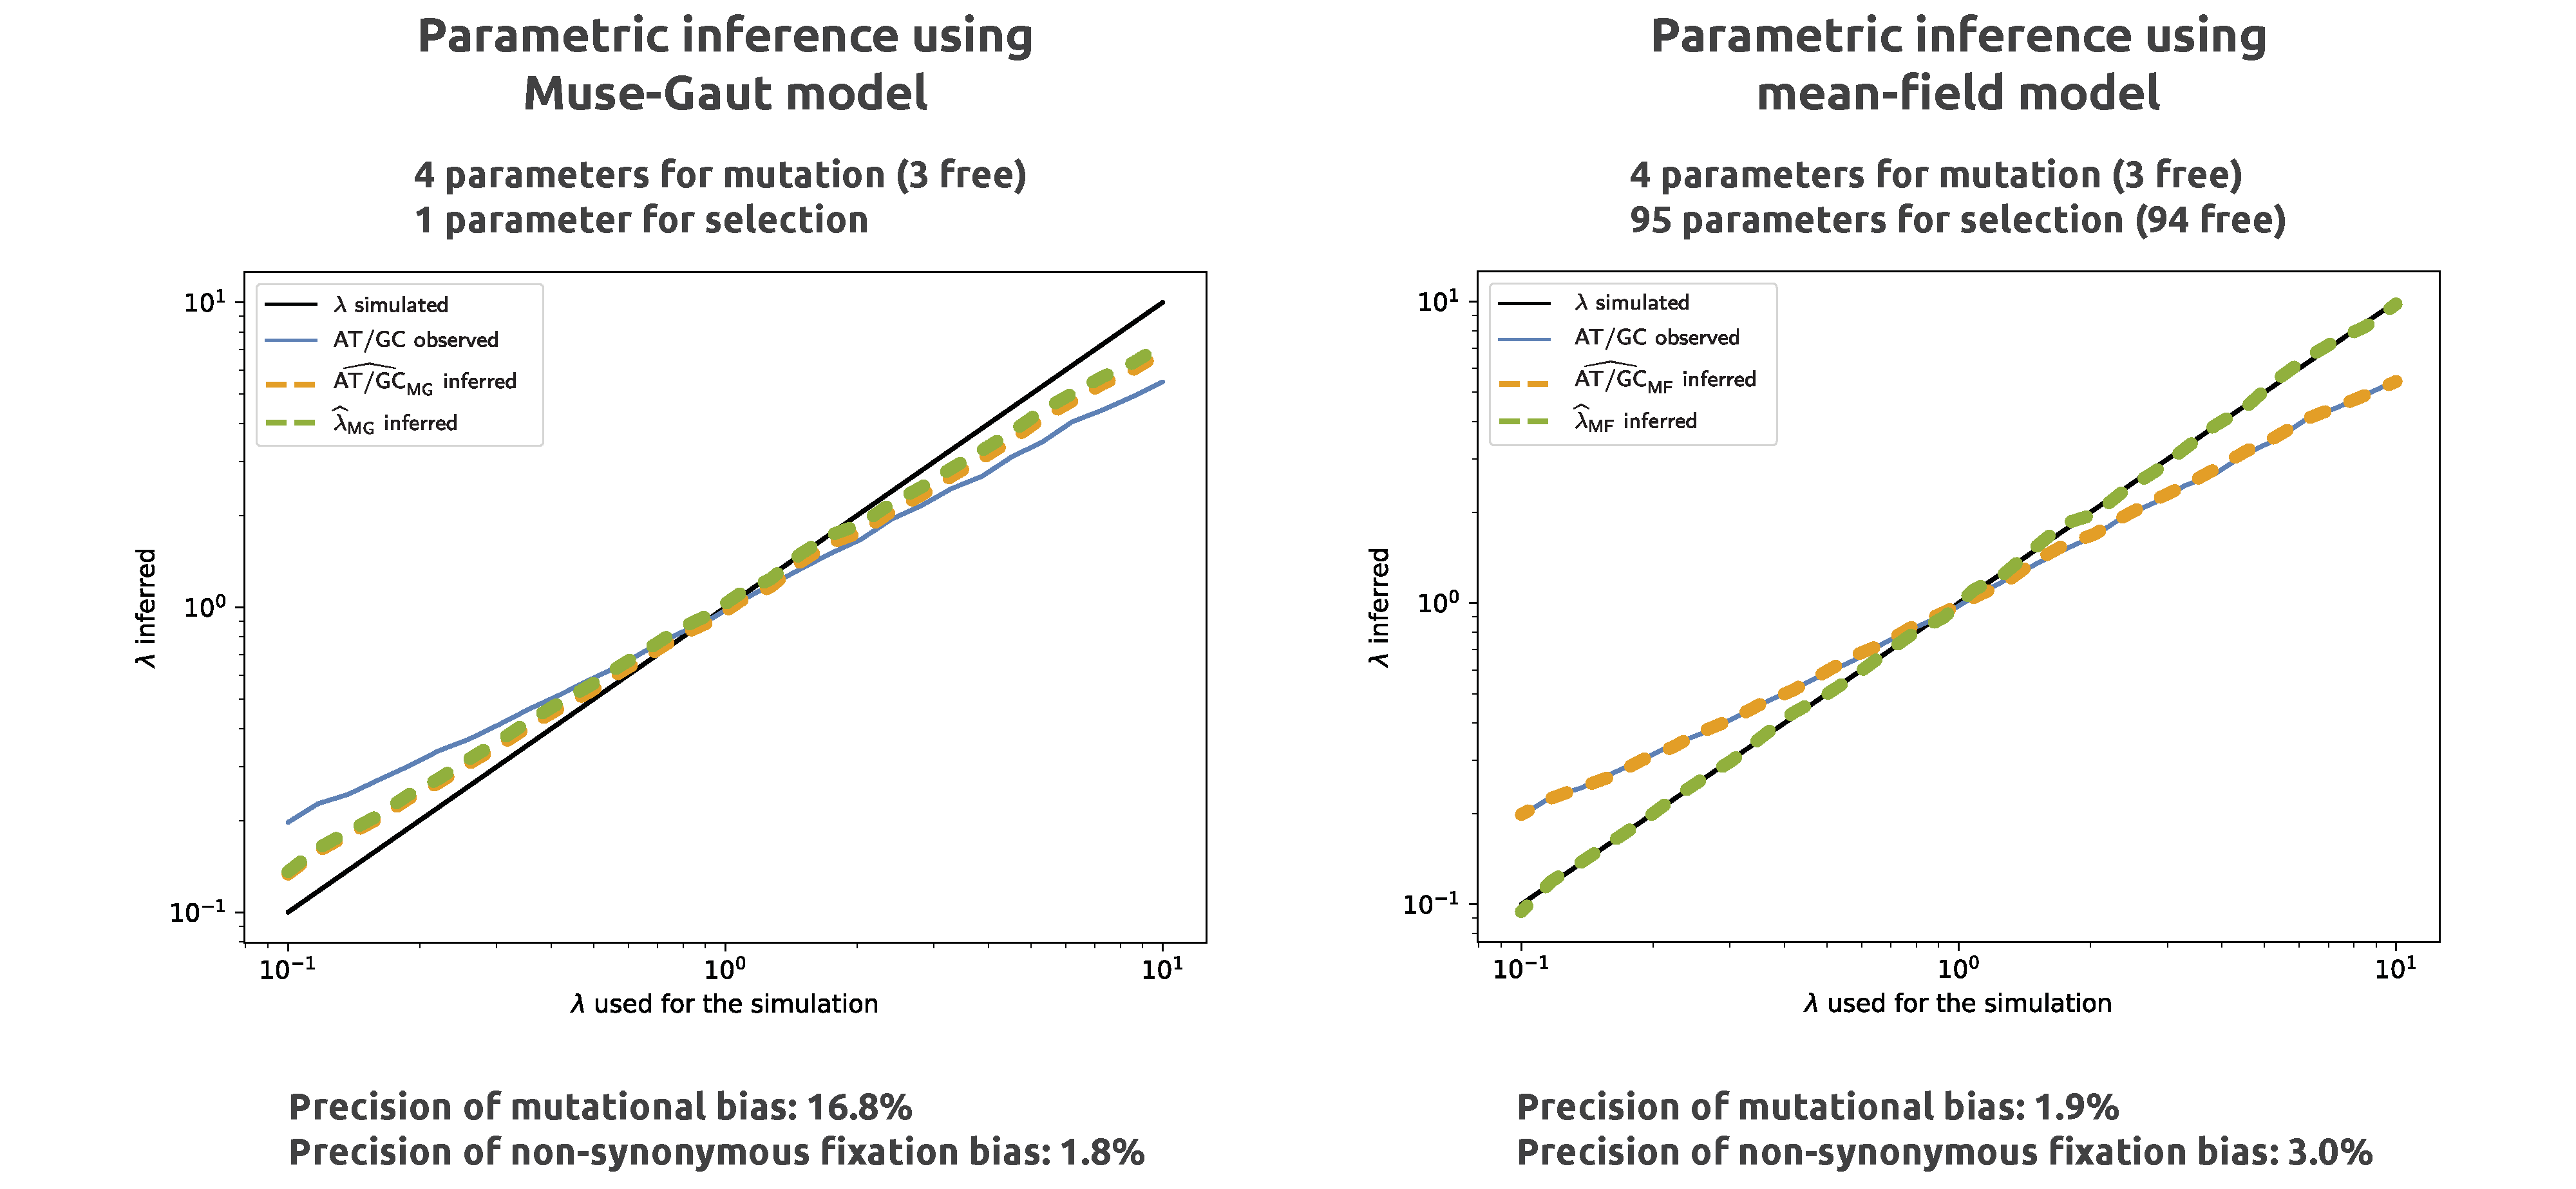
\includegraphics[width=\textwidth] {Simulation-vs-Inference}
    \caption[Estimation of mutation and fixation bias]{
    Estimation of mutation and fixation bias.
    Modeling a single fixation bias leads to skewed estimation of mutation bias.
    Modeling multiple fixation bias leads to precise estimation of mutation bias.
    Estimation of fixation bias doesn't depend on the underlying mutation bias.}
\end{figure}

\begin{table}[H]
    \centering
    \noindent\adjustbox{max width=\textwidth}{%
    \begin{tabu}{|c||c|c|}
        \hline
        \textbf{Estimated parameter} & Nucleoprotein & Lactamase \\
        \hline \textbf{AT/GC of the alignment} & 1.15 & 0.79 \\
        \hline \textbf{Muse-Gaut mutational bias $\left({\widehat{\lambda}_{\text{MG}}} \right)$ } & 1.39 & 0.85 \\
        \hline \textbf{Mean-field mutational bias $\left({\widehat{\lambda}_{\text{MF}}} \right)$} & 1.64 & 0.68 \\
        \hline \textbf{Mean-field fixation bias from AT to GC $\left(\widehat{\omega}_{\textbf{AT} \rightarrow \textbf{GC}}\right)$} & 0.14 & 0.31 \\
        \hline \textbf{Mean-field fixation bias from GC to AT $\left(\widehat{\omega}_{\textbf{GC} \rightarrow \textbf{AT}}\right)$} & 0.10 & 0.44 \\
        \hline
    \end{tabu}}
    \caption[Estimated parameters]{
    Nucleoprotein alignment of 498 amino-acids available for 180 species (left column).
    Lactamase alignment of 263 amino-acids available for 85 species (right column).
    }
\end{table}

The observed composition of the alignment is the result of the articulation between mutation and selection.
Mutational bias is balanced by a fixation bias (selection) in the opposite direction, potentially a confounding effect with gBGC.
Inference of mutational bias requires to model fixation bias in different direction.
Our mean-field parametric framework is not site-wise, but can be used to untangle mutation and selection, potentially in the presence of fluctuating selection or epistasis.


\section{Materials \& Methods}

\subsection{Modeling mutational bias}
\label{sec:mutBias}
The mutation rate between nucleotides is always proportional to $\mu$.
Moreover, mutations from any nucleotide to another weak nucleotide is increased by the factor $\lambda$ compared with mutations to another strong nucleotides.
The rate at which a nucleotide doesn't change is given such the sum of all rates is zero.
The mutation rate matrix is:
\begin{equation}
    \label{nucMatrix}
    \Mutmatrix =
    \begin{pmatrix}
    {-\mu(2 + \lambda)}
        & {\mu} & {\mu} & {\mu \lambda} \\
        {\mu \lambda} & {-\mu(1 + 2\lambda)} & {\mu} & {\mu \lambda} \\
        {\mu \lambda} & {\mu} & {-\mu(1 + 2\lambda)} & {\mu \lambda} \\
        {\mu \lambda} & {\mu} & {\mu} & {-\mu(2 + \lambda)}
    \end{pmatrix}.
\end{equation}
The stationary distribution $ \Subequi$ must be annihilated by the mutation matrix $\Mutmatrix$, which gives the stationary distribution:
\begin{align}
    \Mutequi \Mutmatrix & = 0, \\
    \iff \Mutequi & = \left( \dfrac{\lambda}{2+2\lambda}, \dfrac{1}{2+2\lambda}, \dfrac{1}{2+2\lambda}, \dfrac{\lambda}{2+2\lambda} \right).
    \label{nucStationarity}
\end{align}
The process is reversible and fulfills detailed balance conditions for any pair of different nucleotides:
\begin{align}
    \mutequi_a \mutmatrix_{a, b} =\mutequi_b \mutmatrix_{b, a}.
    \label{nucMutBalance}
\end{align}
It is important to note that ratio of weak over strong nucleotides frequency at stationarity is equal to $\lambda$:
\begin{align}
    \label{lambda}
    \dfrac{ \mutequi_A + \mutequi_T }{ \mutequi_C + \mutequi_G }
    & = \dfrac{ \lambda ( 2 + 2 \lambda)^{-1} + \lambda ( 2 + 2 \lambda)^{-1}}{ ( 2 + 2 \lambda)^{-1} +  ( 2 + 2 \lambda)^{-1}}, \ \textrm{from eq.}\ \ref{nucStationarity},\\
    & = \lambda.
\end{align}

\subsection{Modeling selection at the amino-acid level}
The mutation rate between a pair of \glspl{codon} is given by the underlying mutation rates between nucleotides.
However the rate mutation rate is null if the pair of \glspl{codon} differs by more than one nucleotide:
To note, the \gls{substitution} rate between \glspl{codon} would be equal to the mutation rate if \glspl{codon} are selectively \gls{neutral}.
However, we subsequently take into the selection acting on \gls{codon} by modeling it at the amino-acid level, where each amino-acid $\aai$ encoded by codon $\ci $are given a fitness ($\Fiti$).
By modeling fitness at the amino-acid level, we assume that all \glspl{codon} encoding for one particular amino-acid are selectively \gls{neutral}.
In this modeling framework, the genetic code is of particular importance since the number of \glspl{codon} encoding for a particular amino-acid varies greatly.
As an example, Tryptophan is encoded by one \gls{codon}, while Leucine is encoded by 6 \glspl{codon}.
Intuitively, this variation makes the mutation bias more effective in \glspl{codon} encoding for many amino-acids since there are many mutations possible that are selectively \gls{neutral} (same amino-acid).
While the other hand, the mutation bias is more constrained if the amino-acid is encoded by a few \glspl{codon} since there is only a few mutations possible that are selectively \gls{neutral}.\\

To take into account the heterogeneity of selection between different sites of the protein, we assume that each site $\site$ of the sequence is evolving under a different fitness landscape ($\Fiti\siteexp$).
At one particular site, under a static fitness landscape, the \gls{substitution} rate between \glspl{codon} are given by the product of the mutation rate and the probability of fixation:
\begin{equation}
    \begin{dcases}
        \submatrix_{\itoj} & = 0 \text{ if $\ci$ and $\cj$ are non neighbors} \\
        \submatrix_{\itoj} & = \mu_{\itoj} \text{ if $\ci$ and $\cj$ are syonymous} \\
        \submatrix_{\itoj} & = \mu_{\itoj} \dfrac{\Fitj - \Fiti}{1 - \e^{\Fiti - \Fitj} } \text{ if $\ci$ and $\cj$ are non-syonymous} \\
        \submatrix_{\ci, \ci} & = - \sum_{\cj \neq \ci} \submatrix_{\itoj}
    \end{dcases}
    \label{codonSubRates}
\end{equation}
The stationary distribution $ \Subequi$ must be annihilated by the mutation matrix $\Submatrix$, which gives the stationary distribution at site $\site$:
\begin{align}
    \Subequi\siteexp \bm{Q}\siteexp
    & = 0 ,\\
    \iff \subequi_{\ci}\siteexp
    & = \mathcal{Z}\siteexp \lambda^{\nbrWeak_{\ci}} \e^{\Fiti\siteexp},\\
    & \mathrm{ where } \ \mathcal{Z}\siteexp = \left( \sum_{\cj=1}^{61} \lambda^{\nbrWeak_{\cj}} \e^{\Fitj\siteexp} \right)^{-1}.
    \label{codonStationarity}
\end{align}

Moreover, the \gls{substitution} process is reversible and fulfills detailed balance conditions at each site $\site$:
\begin{align}
    \subequi_{\ci}\siteexp \submatrix_{\itoj}\siteexp = \subequi_{\cj}\siteexp \submatrix_{y, x}\siteexp .
    \label{codonSubBalance}
\end{align}

\subsection{AT/GC as a function of the mutation-selection model}
The \gls{codon} \gls{substitution} process, at site $\site$, which takes into account mutation and selection, is a function of $\lambda$ and $F\siteexp$.
Moreover this process has stationary distribution $\Subequi\siteexp$.
From this equilibrium frequency of \glspl{codon}, we define $\mathrm{AT_{obs}}$ as the observed stationary distribution of weak nucleotides at site $\site$:
\begin{align}
    \mathrm{AT_{obs}}
    & = \frac{1}{3} \sum_{\ci=1}^{61}  \subequi_{\ci}\siteexp \nbrWeak_{\ci} , \ \textrm{by definition},\\
    & = \frac{\mathcal{Z}\siteexp}{3} \sum_{\ci=1}^{61} \lambda^{\nbrWeak_{\ci}} \e^{\Fiti\siteexp} \nbrWeak_{\ci} , \ \textrm{from eq.} \ \ref{codonStationarity}.
    \label{atPctSite}
\end{align}
As noted in \ref{sec:mutBias}, the mutational process leads to $(\mutequi_A+\mutequi_T)/(\mutequi_C+\mutequi_G) = \lambda$.
Similarly, we denote the observed ratio of weak over strong nucleotide frequency, at site $\site$, as $\lambda_{\mathrm{obs}}\siteexp $:
\begin{align}
    \lambda_{\mathrm{obs}}\siteexp 
    & = \dfrac{\mathrm{AT_{obs}}}{1 - \mathrm{AT_{obs}} }, \ \textrm{by definition},\\
    & = \dfrac{ \sum_{\ci=1}^{61} \lambda^{\nbrWeak_{\ci}} \e^{\Fiti\siteexp} \nbrWeak_{\ci}}{\sum_{\ci=1}^{61} \lambda^{\nbrWeak_{\ci}} \e^{\Fiti\siteexp} (3 - \nbrWeak_{\ci} )}, \ \textrm{from eq.} \ \ref{atPctSite}.
\end{align}
At the sequence level, $\lambda_{\mathrm{obs}} $ is the observed stationary ratio of weak over strong nucleotide frequency:
\begin{align}
    \lambda_{\mathrm{obs}} 
    & = \dfrac{1}{\Nsite} \sum_{\site=1}^{\Nsite} \lambda_{\mathrm{obs}}\siteexp \\
    & = \dfrac{1}{\Nsite} \sum_{\site=1}^{\Nsite} \dfrac{ \sum_{\ci=1}^{61} \lambda^{\nbrWeak_{\ci}} \e^{\Fiti\siteexp} \nbrWeak_{\ci}}{\sum_{\ci=1}^{61} \lambda^{\nbrWeak_{\ci}} \e^{\Fiti\siteexp} (3 - \nbrWeak_{\ci} )}
\end{align}

\subsection{Diversity of {codons} as a function of the mutation-selection model}

The \gls{codon} \gls{substitution} process, at site $\site$, which takes into account mutation and selection, is a function of $\lambda$ and $F\siteexp$.
Moreover this process has stationary distribution $\Subequi\siteexp$.
From this equilibrium frequency of \glspl{codon}, we can compute the effective number of \gls{codon}, mathematically this correspond to the diversity of the distribution $\entropy\siteexp$, at site $\site$:
\begin{align}
    \entropy\siteexp
    & = \e^{ - \sum_{\ci=1}^{61}   \subequi_{\ci}\siteexp \ln (  \subequi_{\ci}\siteexp )}, \ \textrm{by definition},\\
    & = \e^{ - \sum_{\ci=1}^{61}   \subequi_{\ci}\siteexp \ln \left( \mathcal{Z}\siteexp \lambda^{\nbrWeak_{\ci}} \e^{\Fiti\siteexp} \right)}, \ \textrm{from eq.} \ \ref{codonStationarity},\\
    & = \e^{ - \sum_{\ci=1}^{61}   \subequi_{\ci}\siteexp \left[ \ln ( \mathcal{Z}\siteexp )+ \ln( \lambda^{\nbrWeak_{\ci}} ) + \ln (\e^{\Fiti\siteexp}) \right] }\\
    & = \e^{ - \ln ( \mathcal{Z}\siteexp ) \sum_{\ci=1}^{61}   \subequi_{\ci}\siteexp } \e^{ -  \ln (\lambda) \sum_{\ci=1}^{61}   \subequi_{\ci}\siteexp \nbrWeak_{\ci} }\e^{ - \sum_{\ci=1}^{61}   \subequi_{\ci}\siteexp \Fiti\siteexp  } \\
    & = \frac{1}{\mathcal{Z}\siteexp} \e^{ -  \ln (\lambda) \sum_{\ci=1}^{61}   \subequi_{\ci}\siteexp \nbrWeak_{\ci} }\e^{ - \sum_{\ci=1}^{61}   \subequi_{\ci}\siteexp \Fiti\siteexp  }
    \label{eq:sit-entropy}
\end{align}

\begin{align}
  \entropy & = \dfrac{1}{\Nsite} \sum_{\site=1}^{\Nsite} \entropy\siteexp\\
	& = \dfrac{1}{\Nsite} \sum_{\site=1}^{\Nsite} \frac{1}{\mathcal{Z}\siteexp} \e^{ -  \ln (\lambda) \sum_{\ci=1}^{61}   \subequi_{\ci}\siteexp \nbrWeak_{\ci} }\e^{ - \sum_{\ci=1}^{61}   \subequi_{\ci}\siteexp \Fiti\siteexp  }
	\label{entropy}
\end{align}

\subsection{dN/dS as a function of the mutation-selection model}

The \gls{codon} \gls{substitution} process, at site $\site$, which takes into account mutation and selection, is a function of $\lambda$ and $F\siteexp$.
Moreover this process has stationary distribution $\Subequi\siteexp$.
From this equilibrium frequency of \glspl{codon}, we define $L_{\NonSyn}$ as the \gls{non-synonymous} flow, at site $\site$:
\begin{align}
    L_{\NonSyn}
    & = \sum_{\ci=1}^{61} \sum_{y \in \NxNonSyn}  \subequi_{\ci}\siteexp \submatrix_{\itoj}\siteexp, \ \textrm{by definition},\\
    & = \sum_{\ci=1}^{61} \sum_{y \in \NxNonSyn} \mathcal{Z}\siteexp \lambda^{\nbrWeak_{\ci}} \e^{\Fiti\siteexp} U_{\itoj} \dfrac{\Fitj\siteexp - \Fiti\siteexp}{1 - \e^{\Fiti\siteexp - \Fitj\siteexp}}, \ \textrm{from eq.}\ \ref{codonSubRates} \ \text{and} \ \ref{codonStationarity},\\
    & = \mathcal{Z}\siteexp \sum_{\ci=1}^{61} \lambda^{\nbrWeak_{\ci}} \sum_{y \in \NxNonSyn}  U_{\itoj} \dfrac{\Fitj\siteexp - \Fiti\siteexp}{\e^{-\Fiti\siteexp} - \e^{ - \Fitj\siteexp}}.
    \label{subFlowNonSyn}
\end{align}
Moreover, we define $K_{\NonSyn}$ as the non-synonymous mutation flow, at site $\site$:
\begin{align}
    K_{\NonSyn}
    & = \sum_{\ci=1}^{61} \sum_{y \in \NxNonSyn}  \subequi_{\ci}\siteexp U_{\itoj}, \ \textrm{by definition},\\
    & = \mathcal{Z}\siteexp  \sum_{\ci=1}^{61} \lambda^{\nbrWeak_{\ci}} \sum_{y \in \NxNonSyn} \e^{\Fiti\siteexp} U_{\itoj}, \ \textrm{from eq.}\ \ref{codonSubRates} \ \text{and} \ \ref{codonStationarity}.
    \label{mutFlowNonSyn}
\end{align}
We also define the mutation and \gls{substitution} synonymous as $K_{\Syn}$ and $L_{\Syn}$ respectively:
\begin{align}
    L_{\Syn}
    & =  \sum_{\ci=1}^{61} \sum_{y \in \NxSyn}  \subequi_{\ci}\siteexp \submatrix_{\itoj}\siteexp, \ \textrm{by definition},\\
    & = \sum_{\ci=1}^{61} \sum_{y \in \NxSyn} \mathcal{Z}\siteexp \lambda^{\nbrWeak_{\ci}} \e^{\Fiti\siteexp} U_{\itoj}, \ \textrm{from eq.}\ \ref{codonSubRates} \ \text{and} \ \ref{codonStationarity}, \\
    & = K_{\Syn}
    \label{subFlowSyn}
\end{align}
Following Spielman and Wilke \citep{Spielman2015}, the rate of non-synonymous to \gls{synonymous} is thus :
\begin{align}
    \omega
    & = \dfrac{L_{\NonSyn}}{K_{\NonSyn}}  \left( \dfrac{L_{\Syn}}{K_{\Syn}}  \right)^{-1}, \\
    & = \dfrac{L_{\NonSyn}}{K_{\NonSyn}}, \ \textrm{from eq.}\ \ref{subFlowSyn} \\
    & = \dfrac{ \sum_{\ci=1}^{61} \lambda^{\nbrWeak_{\ci}} \sum_{y \in \NxNonSyn}  U_{\itoj} \dfrac{\Fitj\siteexp - \Fiti\siteexp}{\e^{ - \Fitj\siteexp} -  \e^{- \Fiti\siteexp} } }{ \sum_{\ci=1}^{61}  \lambda^{\nbrWeak_{\ci}} \sum_{y \in \NxNonSyn} U_{\itoj} \e^{\Fiti\siteexp} }, \ \textrm{from eq.}\ \ref{subFlowNonSyn} \ \text{and} \ \ref{mutFlowNonSyn}.
    \label{omegaSite}
\end{align}
The non-synonymous over synonymous rate for the whole sequence is then given by:
\begin{align}
    \omega
    & = \dfrac{\sum_{\site=1}^{\Nsite} L_{\NonSyn}}{\sum_{\site=1}^{\Nsite}K_{\NonSyn}}  \left( \dfrac{\sum_{\site=1}^{\Nsite}L_{\Syn}}{\sum_{\site=1}^{\Nsite}K_{\Syn}}  \right)^{-1}, \\
    & = \dfrac{\sum_{\site=1}^{\Nsite} L_{\NonSyn}}{\sum_{\site=1}^{\Nsite}K_{\NonSyn}}, \ \textrm{from eq.}\ \ref{subFlowSyn} \\
    & = \dfrac{ \sum_{\site=1}^{\Nsite} \sum_{\ci=1}^{61} \lambda^{\nbrWeak_{\ci}} \sum_{y \in \NxNonSyn}  U_{\itoj} \dfrac{\Fitj\siteexp - \Fiti\siteexp}{\e^{ - \Fitj\siteexp} -  \e^{- \Fiti\siteexp} } }{ \sum_{\site=1}^{\Nsite} \sum_{\ci=1}^{61}  \lambda^{\nbrWeak_{\ci}}  \sum_{y \in \NxNonSyn} U_{\itoj} \e^{\Fiti\siteexp}}, \ \textrm{from eq.}\ \ref{subFlowNonSyn} \ \text{and} \ \ref{mutFlowNonSyn}.
    \\
    & = \dfrac{ \sum_{\ci=1}^{61} \lambda^{\nbrWeak_{\ci}} \sum_{y \in \NxNonSyn}  U_{\itoj}  \sum_{\site=1}^{\Nsite} \dfrac{\Fitj\siteexp - \Fiti\siteexp}{\e^{ - \Fitj\siteexp} -  \e^{- \Fiti\siteexp} } }{  \sum_{\ci=1}^{61}  \lambda^{\nbrWeak_{\ci}}  \sum_{y \in \NxNonSyn} U_{\itoj}  \sum_{\site=1}^{\Nsite} \e^{\Fiti\siteexp}}.
    \label{omegaSeq}
\end{align}